\documentclass[11pt]{article}
\usepackage[margin=0.78in]{geometry}
\usepackage{amsmath,amssymb,amsthm}
\usepackage{microtype}
\usepackage[htt]{hyphenat}
\usepackage{booktabs}
\usepackage{tabularx}
\usepackage{enumitem}
\usepackage{xcolor}
\usepackage{tikz}
\usetikzlibrary{arrows.meta,positioning}
\usepackage[colorlinks=true,linkcolor=blue!50!black,urlcolor=blue!50!black,citecolor=blue!50!black]{hyperref}

\newcommand{\Lean}[1]{\texttt{\small #1}}
\newcommand{\inarch}[1]{\par{\small\raggedright\noindent\emph{In the archive:} #1\par}}
\newcommand{\Q}{\mathbf{Q}}
\newcommand{\Z}{\mathbf{Z}}
\newcommand{\Sha}{\mathrm{Sha}}
\renewcommand{\Re}{\operatorname{Re}}
\setlist{itemsep=2pt,topsep=4pt}

\title{A Roadmap to the Alp\"oge--Claude Lean Proof\\ of the Riemann Hypothesis}
\date{21 November 2026}
\author{}

\sloppy\emergencystretch=4em
\begin{document}
\maketitle

\begin{abstract}
On 20 November 2026 Levent Alp\"oge announced a proof, found with Claude, of the Riemann hypothesis and of the generalized Riemann hypothesis for Dirichlet $L$-functions. It is a Lean~4 archive of about 17.4 million lines; Andrew Sutherland has checked it with several independent kernels. Read from the top, the argument has a classical shape. A Landau-type positivity argument reduces the theorem to a one-sided bound: a centred, smoothed von Mangoldt sum over prime powers, combined over a family of characters, stays below $x^{1/2+\varepsilon}$ on long windows. That bound is proved in the spirit of Stepanov's method for curves over finite fields, where an auxiliary function vanishing to high order at almost every point, with controlled degree, gives a square-root bound. Over the integers no multiplicity plays that role; the archive manufactures one from a chain of about $\sqrt{x}$ theta lifts between definite unitary groups, which supplies a cumulative lower bound on the $p$-adic valuations of selected periods. Divisibility of unwanted origin, coming from Galois cohomology, is controlled by a bound on Tate--Shafarevich-type groups over a chosen family of CM subfields of cyclotomic fields. The archive also formalizes, in the forms the argument needs, a large body of published theory, from local Langlands to $p$-adic Hodge theory. This note ties each step to declarations of the archive and lists the points that remain to be traced.
\end{abstract}

\paragraph{About this note.} Its author set the direction and made the editorial decisions; the text was written and cross-checked with several AI models, including Claude, a model developed by Anthropic, where Alp\"oge works. Facts about the archive come from reading its source (version with SHA-256 \Lean{9631b4f0\ldots c7fc}, the one checked by Sutherland); facts about verification come from Sutherland's report \cite{sutherland}. Explanations of mathematical intent are ours; Section~\ref{sec:open} lists the places where we have traced the statements and the proofs remain to be read.

\section{Status}
As of Sutherland's report (snapshot 2026-11-21 10:05 UTC) \cite{sutherland}: all 175{,}187 modules compile with no errors; the five main theorems depend only on \Lean{propext}, \Lean{Classical.choice} and \Lean{Quot.sound}; \Lean{leanchecker} replays every module; the exported environment is accepted by nanoda and by con-leche, and lean4lean accepts every module. The replay of the export by Lean's default and paranoid kernels is running, and so is an end-to-end \Lean{lake comparator} run, whose statement comparison and axiom check have passed. Sutherland has also joined the proof to an independent formalization of Robin's and Lagarias's criteria \cite{robin1984}. The joined proof, accepted by nanoda and con-leche, gives $\sigma(n) < e^{\gamma} n \log\log n$ for every $n > 5040$ and $\sigma(n) \le H_n + e^{H_n}\log H_n$ for every $n \ge 1$, statements about divisor sums and harmonic numbers alone. Alp\"oge writes that he has not yet mastered the surrounding mathematics \cite{alpoge}; Tao describes the GRH argument, on a very preliminary reading, as using the full power of the Langlands programme and arithmetic geometry \cite{tao}.

\section{The statements}
\Lean{Main.lean} proves five theorems. The first is Mathlib's \Lean{RiemannHypothesis}:
\[
\forall s\in\mathbf C,\quad \zeta(s)=0,\ \ s\notin\{-2,-4,\dots\},\ \ s\neq 1\ \Longrightarrow\ \Re s=\tfrac12 .
\]
The second restates it. The other three concern Dirichlet characters $\chi$ of any modulus $N\ge1$, through Mathlib's \Lean{DirichletCharacter.LFunction}: $L(s,\chi)\ne0$ for $\Re s>1/2$ (excluding $s=1$ for principal $\chi$, where $L$ has a pole); every zero with $0<\Re s<1$ lies on $\Re s=1/2$; and the same for primitive $\chi$. Dedekind zeta functions of general number fields are not covered.

\begin{figure}[t]
\centering
\resizebox{\linewidth}{!}{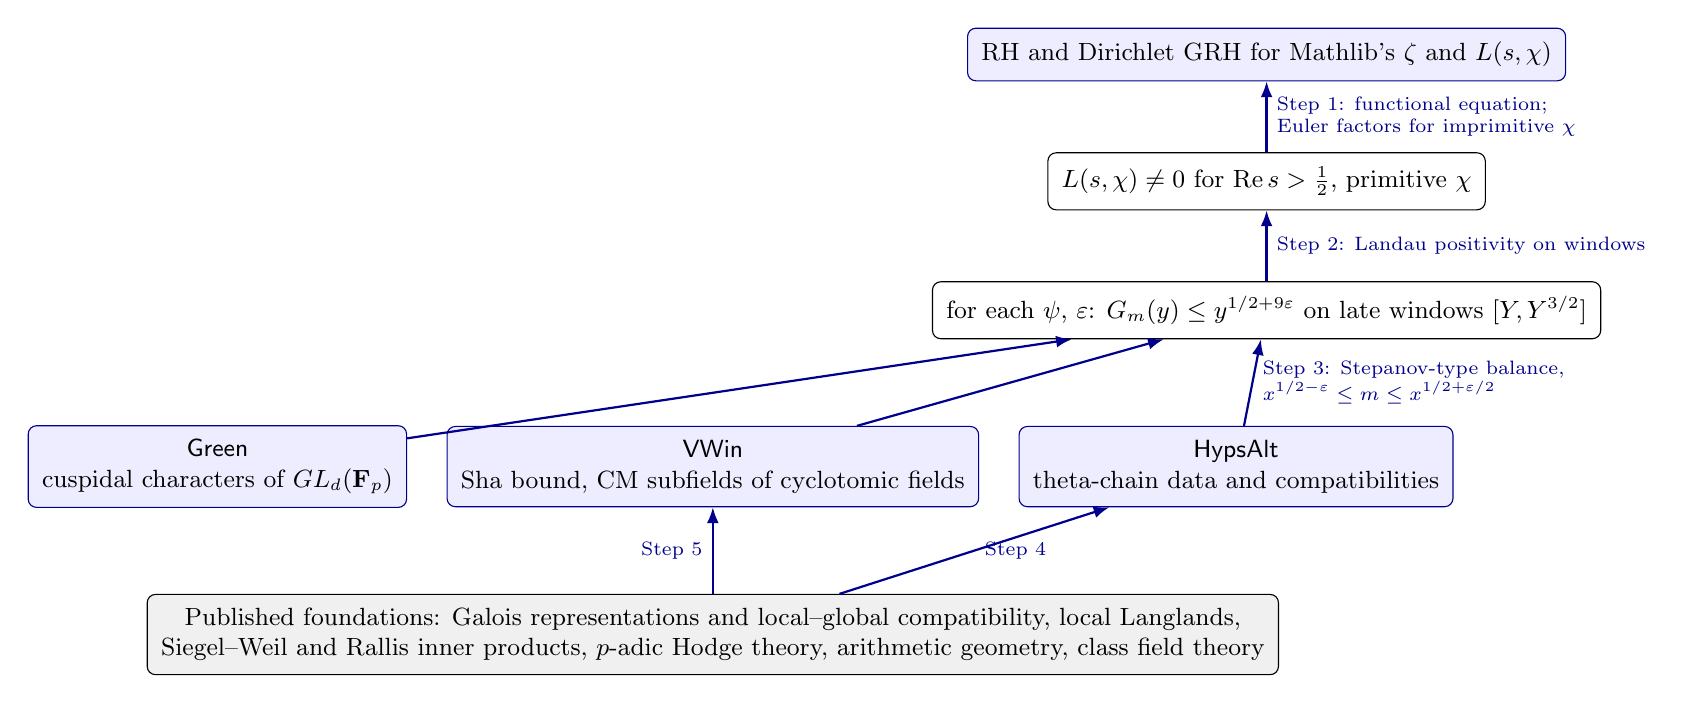
\begin{tikzpicture}[
  box/.style={draw, rounded corners=3pt, align=center, font=\small, inner sep=5pt, minimum width=36mm},
  hi/.style={box, fill=blue!7, draw=blue!55!black},
  base/.style={box, fill=black!6},
  arr/.style={-{Latex[length=2mm]}, blue!55!black, thick},
  lab/.style={font=\scriptsize, text=blue!55!black, align=left}]
\node[hi] (rh) {RH and Dirichlet GRH for Mathlib's $\zeta$ and $L(s,\chi)$};
\node[box, below=9mm of rh] (every) {$L(s,\chi)\ne0$ for $\Re s>\tfrac12$, primitive $\chi$};
\node[box, below=9mm of every] (gm) {for each $\psi$, $\varepsilon$: $G_m(y)\le y^{1/2+9\varepsilon}$ on late windows $[Y,Y^{3/2}]$};
\node[hi, below left=11mm and -6mm of gm] (vw) {\textsf{VWin}\\ $\Sha$ bound, CM subfields of cyclotomic fields};
\node[hi, left=5mm of vw] (gr) {\textsf{Green}\\ cuspidal characters of $GL_d(\mathbf F_p)$};
\node[hi, right=5mm of vw] (hy) {\textsf{HypsAlt}\\ theta-chain data and compatibilities};
\node[base, below=11mm of vw, minimum width=125mm] (lit) {Published foundations: Galois representations and local--global compatibility, local Langlands,\\ Siegel--Weil and Rallis inner products, $p$-adic Hodge theory, arithmetic geometry, class field theory};
\draw[arr] (every) -- node[lab, right]{Step 1: functional equation;\\ Euler factors for imprimitive $\chi$} (rh);
\draw[arr] (gm) -- node[lab, right]{Step 2: Landau positivity on windows} (every);
\draw[arr] (vw) -- (gm); \draw[arr] (gr) -- (gm); \draw[arr] (hy) -- node[lab, right]{Step 3: Stepanov-type balance,\\ $x^{1/2-\varepsilon}\le m\le x^{1/2+\varepsilon/2}$} (gm);
\draw[arr] (lit) -- node[lab, left]{Step 5} (vw);
\draw[arr] (lit) -- node[lab, right]{Step 4} (hy);
\end{tikzpicture}}
\caption{The top of the proof, read from the bottom. Shaded blue: the top statement and the three inputs of the reduction (\textsf{Green} is a classical theorem). Grey: published theory, formalized in the forms the argument needs. Size: the archive-local import closure of \Lean{TopPlug}, from the three inputs to all Dirichlet characters, has 17{,}276 of the 175{,}187 files (3.0 million lines).}
\label{fig:map}
\end{figure}

\section{Step 1: it suffices to look to the right of $1/2$}\label{sec:s1}
It is enough to prove $L(s,\chi)\neq0$ for $\Re s>1/2$ and every $\chi$ (excluding the pole at $s=1$ of principal characters). For primitive $\chi$, the functional equation relates $L(s,\chi)$ to $L(1-s,\overline\chi)$ with a non-zero root number, and the archimedean Gamma factor is holomorphic and non-vanishing for $\Re s>0$; this reflects zeros in $0<\Re s<1/2$ to $1/2<\Re s<1$. (Mathlib's \Lean{RiemannHypothesis} also covers $\Re s\le0$, where the same equation leaves only the trivial zeros.) Imprimitive $L$-functions modulo $N$ are primitive ones times the Euler factors $1-\chi^*(p)p^{-s}$ for $p\mid N$, which do not vanish for $\Re s>0$. The Riemann hypothesis is the case of the trivial character modulo $1$, whose $L$-function is $\zeta$.

\inarch{\Lean{Formalism.VW.critLine}, \Lean{Formalism.VW.rh\_of\_every} (file \Lean{Formalism/GammaFactorNonvanishing/CritLine.lean}); \Lean{UpperTheory.Top.imprimitive}; the intermediate property is \Lean{UpperTheory.EveryCharacter}.}

\section{Step 2: it suffices to bound a prime count from above}\label{sec:s2}
Fix a primitive character $\psi$ of order $o$ and let $\mathcal X$ be the set of the $o$ primitive characters inducing the powers of $\psi$; it is closed under complex conjugation. With the von Mangoldt function $\Lambda(n)$, put
\[
G_z(y)=\sum_{n\le y}\Lambda(n)\Bigl(\frac yn-1\Bigr)-y\log y+(1+\gamma)y,\qquad
g_\chi(y)=\sum_{n\le y}\Lambda(n)\chi(n)\Bigl(\frac yn-1\Bigr)+y\,\frac{L'(1,\chi)}{L(1,\chi)}\ \ (\chi\ne1),
\]
\[
G_m(y)=G_z(y)+\frac1{3o+1}\sum_{\chi\in\mathcal X,\ \chi\ne1}\Re g_\chi(y).
\]
The formula for $G_z$ is equivalent to item~5 of Alp\"oge's timeline \cite{alpoge}. Because $\bigl|\sum_{\chi\ne1}\Re\chi(n)\bigr|<3o+1$, the arithmetic part of $G_m$ has non-negative coefficients. Landau showed in 1905 that a Dirichlet series with non-negative coefficients and finite abscissa of convergence has a singularity at the real point of that abscissa \cite{landau}. In the archive, a zero $\rho$ of some $L(s,\chi)$, $\chi\in\mathcal X$, gives a simple pole with non-zero residue at $\rho$ of the Laplace transform of $u\mapsto G_m(e^u)$. From this the archive proves a window version: \emph{if $0<\theta<1$ and for every $Y_0$ there is $Y\ge Y_0$ with $G_m(y)\le y^\theta$ on the whole interval $[Y,Y^{3/2}]$, then no $L(s,\chi)$ with $\chi\in\mathcal X$ vanishes for $\Re s>\theta$.} The problem thus becomes a one-sided estimate: $G_m(y)\le y^{1/2+O(\varepsilon)}$ on such windows, for every small $\varepsilon>0$.

\inarch{$G_z$ in \Lean{Formalism/StatementOC.lean}; $G_m$ and the proposition \Lean{ChebyshevGrowthImpliesZeroFree} in \Lean{.../TotientGaloisClasses/\-ExplicitFormulaError\-OfHostConditions.lean}; an everywhere-eventually version in \Lean{Landau.lean:538}; the window version used in the final proof in \Lean{PrimitiveCosets/Imports.lean}, \Lean{ZeroFreeOfRpowWindow.lean} and \Lean{landauWindow.lean}.}

\section{Step 3: a Stepanov-type balance}\label{sec:s3}
Alp\"oge calls the argument a descendant of Stepanov's method \cite{alpoge}. Over a finite field, Stepanov \cite{stepanov} and Bombieri \cite{bombieri} bound the number of points on a curve by building a non-zero rational function on the curve that vanishes to order at least $m$ at all but $m_0$ of the $N$ rational points and has a pole divisor of degree $D$, so that $m(N-m_0)\le D$. The Frobenius map forces the vanishing without locating the points; with $m$ of size $\sqrt q$ and $D/m=q+O(\sqrt q)$ this gives $N\le q+O(\sqrt q)$, and extensions or twists give the lower bound. Over $\Z$ there is no derivative, and, as Alp\"oge puts it, it is hard to find a multiplicity that plays the same role in this estimate. The archive replaces it by a chain of $m$ theta lifts (Step 4). The estimate is organized as follows.

\begin{itemize}
\item At every large point $x$ of a window, a chain of $m$ layers is built; the different shift positions share one family of top integer weights (local weights may vary with the layer).
\item For each layer there is an exact identity: a weighted sum over prime powers, minus a main term, equals a Fourier sum on a finite abelian group. Passing to the common weights produces a controlled comparison error.
\item Summing over the $m$ layers and averaging over a subgroup $A_0$ keeps exactly the characters trivial on $A_0$. Writing $G=G_{m,A}-\Sigma_A$ (the subscript of $G_m$ is a label, unrelated to the chain length $m$), where $\Sigma_A=\sum_\psi|G_\psi(x)|$ runs over the characters trivial on $A_0$ outside the retained set, one obtains, with $Q=n_T\,m\,b$ and $\delta=n_{T2}/n$,
\[
Q\cdot\frac\delta2\cdot\bigl(G-4x^{1/2+\varepsilon}\bigr)\le E+\frac{2Q}{x}.
\]
\item A geometric estimate bounds $E$ by $x^{C\varepsilon}$ times a sum of four terms. After dividing the bracket by $Q$, the first is at most $2x/m$, which the lower bound $m\ge x^{1/2-\varepsilon}$ controls; the third grows with $m$ and needs the upper bound $m\le x^{1/2+\varepsilon/2}$; the second and fourth use bounds on a rank parameter $k$ and on set sizes. In total $E/Q\le 10\,x^{C\varepsilon}x^{1/2+13\varepsilon/8}$ with $C=e_D+e_L+3$.
\item The characters in $\Sigma_A$ are the at most $4o$ characters trivial on $A_0$ outside the retained set; each is a power of $\psi$ times a non-trivial quadratic twist $(\frac{\cdot}{q})^i(\frac{\cdot}{d})^j$ by two auxiliary primes. For every window the archive chooses $q,d$ so that all these twisted sums satisfy $|g_\chi(y)|\le y^{1/2+\varepsilon/2}$ on the whole window, using a mean-square estimate over candidate primes and a zero-density estimate, both proved in the archive (\Lean{QH.pairEx}); no bound for $\mathcal X$ is used here. With $\Sigma_A\le 4o\,x^{1/2+\varepsilon}$ (\Lean{sigA\_le}) and $\delta\ge x^{-\varepsilon}$ this yields $G_m(x)\le x^{1/2+(e_D+e_L+7)\varepsilon}$. The construction used takes $e_D=2$, $e_L=0$, so $G_m(x)\le x^{1/2+9\varepsilon}$ on the windows. Given a zero with $\Re s>1/2$, choosing $\varepsilon$ small and applying Step~2 gives a contradiction.
\end{itemize}

After the main term has been subtracted, the first term $2x/m$ plays the role of ``degree divided by multiplicity''. Alp\"oge writes that the chain length of order $\sqrt X$ was Claude's suggestion \cite{alpoge}.

\inarch{\Lean{ChainTied} (\Lean{Formalism/SharpRestriction/GlobalSchurBounds/TieGlobal.lean}); common weights \Lean{LossesSmallShares.lean:86}; the term $4x^{1/2+\varepsilon}$ in \Lean{ChCore.lean}; the four terms in \Lean{LipschitzWeightAndMinimum.lean} (line 522 for $x/m$); $x^{1/2-\varepsilon}\le m$ in \Lean{RestSize} (\Lean{Formalism/SizeWindowBrackets/SChain.lean}); the final count in \Lean{CoreGm.lean}. The three inputs enter through \Lean{UpperTheory.Top.zero\_free\_all\_of\_green\_v\_win} (primitive characters), wrapped by \Lean{every\_character\_of\_green\_v\_win} (all characters), both in \Lean{.../ThirdPlaceSeries/TopPlug.lean}.}

\section{Step 4: multiplicity from theta lifts}\label{sec:s4}
A theta lift transports an automorphic form on one group to an automorphic form on another, by integrating against a theta kernel that is automorphic for both groups. The archive works with definite unitary groups, for which the theta kernel depends on auxiliary splitting characters. In the level, weight and algebraic model chosen there, the relevant automorphic forms are described on finitely many double cosets (classes of lattices), and, for vectors in the specified lattices and eigenspaces, the periods that appear have representatives in a number field, so one can measure their divisibility by a prime.

\begin{itemize}
\item \emph{Layers.} Along a chain $U(X_0)\to U(X_1)\to\dots\to U(X_m)$, each lift contributes a provable net amount at each relevant prime: a local gain (zero at some specified primes) plus a base term minus the denominator loss of that step. The gains add up to a budget $\mathrm{sg}(u,w)=\sum_j(\mathrm{gainD}_j+F_j-E_j)$. The net amount varies from layer to layer.
\item \emph{Divisibility of periods.} For the primes it treats, the archive shows that the period at the end of the chain is represented by an element $y$ of the coefficient field with $y=0$ or $v_w(y)\ge e_w\,\mathrm{sg}(u,w)$, where $v_w$ is normalized by $v_w(\varpi_w)=1$ and $e_w$ is the ramification index of $w$ over $p$; the level primes and two auxiliary primes are handled separately.
\item \emph{Division.} This lower bound allows one to replace the input lattice $\mathrm{NuLat}_u$ by $I_u\,\mathrm{NuLat}_u$, with the fractional ideal $I_u=\prod_w\mathfrak p_w^{-\lfloor e_w\,\mathrm{sg}(u,w)\rfloor}$, while keeping the pairings integral. Divisibility becomes a gain in the slope of a lattice, which enters a height budget and then the error $E$ of Step~3. Item~13 of the timeline mentions the Bost slope inequality \cite{bost}.
\item \emph{Sizes.} The Rallis inner product formula (for unitary groups see \cite{hks}) controls the size of each lift on the relevant isotypic components; the Chowla--Selberg formula \cite{cs} normalizes CM periods through the mean of their logarithms over the complex embeddings; the Siegel mass formula gives volume ratios between consecutive ranks.
\end{itemize}

\inarch{\Lean{FormalGroupSystem.Conclusion2}, \Lean{Conclusion5} (one step and the whole chain); the divisibility bound \Lean{LocalQuadraticParts.adm2}, supplied in the final proof by \Lean{Adm2InU.admissible\_level\_two}; \Lean{BasicNotions.SizeData\textsubscript{2}.sg}; \Lean{DV.Iu}, \Lean{DV.NprimeDef}; the exact slope change \Lean{J.mu\_diff}; the global lattice glued across Hecke characters \Lean{IndefData.RR}.}

\section{Step 5: controlling extra divisibility ($\Sha$ bounds)}\label{sec:s5}
Divisibility of special values can also come from arithmetic objects unrelated to the chain. A classical example is the Herbrand--Ribet theorem: for an odd prime $p$, even $2\le k\le p-3$ and $\omega$ the Teichm\"uller character, $p$ divides the numerator of $B_k$ exactly when the $\omega^{1-k}$-component of the $p$-class group of $\Q(\zeta_p)$ is non-zero (Herbrand \cite{herbrand} proved one direction, Ribet \cite{ribet} the converse). In the archive the corresponding error enters the per-layer divisibility budget as a weighted sum of lengths of Tate--Shafarevich-type groups, which must be bounded.

\paragraph{The fields.} Up to $\Q$-isomorphism, $E=K_\psi\cdot\Q(\zeta_{2^{a+2}})^+\cdot\Q(\sqrt{-q})\cdot\Q(\sqrt{-d})$, where $K_\psi$ is the fixed field of $\ker\psi$. The auxiliary primes satisfy $q\equiv3\pmod 8$, $d\equiv7\pmod{16}$, $q\mid d+1$, every odd prime $p\le U^{\varepsilon/5}$ divides $d+1$ (so these primes split in $\Q(\sqrt{-d})$), and $\log q$, $\log d$ lie in prescribed ranges. Elsewhere a construction of Behrend type \cite{behrend} selects dense sets with few short Frobenius relations.

\paragraph{The groups and the bound.} For a prime $\ell$ and $k\ge1$,
\[
\Sha_{\ell,k}(E)=\ker\Bigl(H^1\bigl(G_{E,S_\ell},\Q_\ell/\Z_\ell(-k)\bigr)\to\prod_{v\mid\ell}H^1\bigl(G_{E_v},\Q_\ell/\Z_\ell(-k)\bigr)\Bigr).
\]
Here $S_\ell$ consists of the places above $\ell$ and $\infty$, and $G_{E,S_\ell}$ is the Galois group of the maximal extension of $E$ unramified outside $S_\ell$. \Lean{VVle E t B} asks that these lengths be finite for $1\le k<t$ and that $\sum_{\ell\in S}\log\ell\sum_{1\le k<t}\operatorname{length}\Sha_{\ell,k}(E)\le B$ for every finite set $S$ of primes (including $\ell=2$). \Lean{VWin} states: for every primitive $\psi$, every $0<\varepsilon<1/52$ and every page function $a:\mathbf R\to\mathbf N$ with $x^{2+8\varepsilon}\le2^{a(x)}\le2x^{2+8\varepsilon}$ for all $x\ge1$, there are $J\ge1$ and $X_0$ such that for every $X\ge X_0$ and every admissible pair $(q,d)$ at scale $U=X^{1/J}$ there is $Y$ with $U\le Y$, $Y^2\le X$, and for every $x\in[Y,Y^2]$ and every field $E$ as above with $a=a(x)$,
\[
\textstyle\text{\Lean{VVle}}\bigl(E,\ \lfloor x^{401}\rfloor,\ \exp(x^{\varepsilon}/2)\bigr).
\]
Downstream, using the existence of admissible prime pairs and rescaling, these windows supply the windows $[Z,Z^{3/2}]$ of Step~2. The exponent comes from a rank estimate: with $Y=x^{1/100}$ a product of bounds is at most $10576\,Y^{39967}$, which is absorbed into $t\le Y^{40000}=x^{400}$; rescaling $x=\lambda x'$ with $x'\ge\lambda^{400}$ then gives $x^{400}\le x'^{401}$.

\paragraph{Proof outline.} The prime $2$ is treated separately; at odd primes the group splits under complex conjugation into two components, which are estimated separately and added. Iwasawa theory along the cyclotomic $\Z_\ell$-extension leaves only finitely many exceptional twists; the scale is chosen so that exceptional twists avoid the middle band $(x^\eta,x^{401}]$, and small exceptional twists are estimated separately. The remaining component is controlled through automorphic representations, base change and deformation theory, with input from Galois representations (\Lean{UpperTheory.One.vwin\_of\_row}). In Step~4 the bound enters as $\sqrt b$ for an exponential scale $b$ and is absorbed by $\sqrt b\le b$. Alp\"oge calls this ``a significant weakening of Vandiver'' and writes that he believes the vanishing of several $K$-groups of $\Z$ follows \cite{alpoge}. Vandiver's conjecture asserts $p\nmid h(\Q(\zeta_p)^+)$ for every prime $p$; Kurihara related it to the $K$-groups of $\Z$ \cite{kurihara}; in its modern form it is equivalent to $K_{4n}(\Z)=0$ for all $n\ge1$ \cite{weibel}. The archive contains no formal implication between \Lean{VWin} and Vandiver's conjecture; the comparison appears in the remark.

\inarch{\Lean{VWin}, \Lean{VWinAt}, \Lean{VVle}, \Lean{IsChiField}, \Lean{WinPair} in \Lean{CharacterBoxes/ExistsPageN.lean}; \Lean{Formalism.GaloisCohomology.shaLen}; \Lean{divinN\_of\_hypV} in \Lean{DivinNOfHypV.lean}; \Lean{WinPairs.lean} for the rescaling.}

\section{The foundations}\label{sec:found}
A summary file lists 185 single entries through which literature statements reach the final proof (176 named \Lean{\_of\_literature}); the final proof uses the archive's own proof terms for them. One slot is a placeholder and another entry forwards its first argument, so fewer distinct published theorems are involved. Representative areas and standard sources for the relevant theory follow; the versions used are those stated in each entry.

\medskip
\noindent\begin{tabularx}{\linewidth}{@{}lX@{}}
\toprule
Area & Representative theory and sources\\
\midrule
Galois representations & $\ell$-adic representations attached to regular algebraic polarized cuspidal representations \cite{shin}; local--global compatibility \cite{caraiani12,caraiani14,ty}; Clozel's cohomologicality and purity\\
Local Langlands & $GL_n$ over $p$-adic fields \cite{ht,henniart}; Bernstein--Zelevinsky theory\\
Theta correspondence & Weil representation and Howe duality; Siegel--Weil; Rallis inner products \cite{rallis}; doubling \cite{psr}\\
$p$-adic Hodge theory & Fontaine's period rings; de Rham implies potentially semistable; prismatic cohomology \cite{bs}; Grothendieck--Messing\\
Arithmetic geometry & semistable reduction of abelian varieties; toroidal compactifications; arithmetic Hilbert--Samuel and heights; Kawamata--Viehweg and Nadel vanishing; resolution of singularities\\
Galois cohomology & Poitou--Tate; Greenberg--Wiles; local Tate duality\\
Class field theory, $L$-functions & Artin reciprocity; Chebotarev (degree-one primes); Hasse norm theorem; complex multiplication; Hecke--Tate functional equations; Deligne--Ribet; Linnik\\
Representation theory & characters of $GL_d(\mathbf F_q)$ \cite{green}; discrete series; Casselman--Wallach; Jacquet--Shalika\\
\bottomrule
\end{tabularx}

\medskip
The archive-local import closure of \Lean{TopPlug} (three inputs $\Rightarrow$ every character) has 17{,}276 files and about 3.0 million lines; the directory \Lean{Development/AbelianVarietyTheory} alone has 99{,}187 of the 175{,}187 files.

\section{Points still to be traced}\label{sec:open}
\begin{itemize}
\item The local computation behind each layer's gain in Step~4, and the upstream theta-kernel and period identities behind each row of $E$ in Step~3.
\item The route that, by item~14 of the timeline, stopped at $2/3$ without division. The final archive does not contain it.
\item The internals of the hard component of the $\Sha$ bound (Kato's Euler system, deformation rigidity at automorphic symplectic points of dimension four, an $R=T$ statement over $\Q(i)$) below the first two levels.
\item The forms in which published theorems are proved. The archive proves the Galois-representation and local-Langlands statements it needs in weakened forms: partial local--global compatibility, and a local correspondence pinned down only on a restricted class of representations. Full versions are stated in the archive and not used by the final proof.
\item Whether the integral-bound version of the window criterion proved in Step~2 appears in the literature; the pointwise version is close to Kaczorowski and Pintz \cite{kp}.
\end{itemize}
Sutherland's report records kernel acceptance of the formal proof and a comparison of the five target statements by \Lean{con-leche --compare}. The points above concern a human-readable account of the intermediate argument, and a written version of normal length.

\section{Lean companion}
The repository accompanying this note contains \Lean{Roadmap.lean}, which restates the top of the proof with the archive's own theorems and proves, inside the archive,
\[
\Lean{Green}\ \wedge\ \Lean{VWin}\ \wedge\ \Lean{Nonempty (HypsAlt \dots)}\ \Longrightarrow\ \Lean{RiemannHypothesis}.
\]
Compiled against the archive, \Lean{Roadmap.rh\_of\_three\_inputs} depends only on \Lean{propext}, \Lean{Classical.choice} and \Lean{Quot.sound}. The archive carries no licence; the README explains how to download it from \url{https://alpo.ge}, check its SHA-256 and build the file.

\begin{thebibliography}{99}\footnotesize\setlength{\itemsep}{0pt}
\bibitem{alpoge} L.~Alp\"oge, \emph{[remark on a proof of RH and GRH]}, 20 November 2026, \url{https://alpo.ge/remark.pdf}; Lean archive \url{https://alpo.ge/lean.tar.gz.part01}--\Lean{part14}.
\bibitem{sutherland} A.~V.~Sutherland, \emph{Verification files for the Lean proof of the Riemann Hypothesis}, \url{https://math.mit.edu/~drew/grh/}, updated 2026-11-21 10:05 UTC.
\bibitem{robin1984} kimihiro64, \emph{Robin1984: a Lean~4 formalization of Robin's 1984 criterion}, \url{https://github.com/kimihiro64/Robin1984}, commit \Lean{acab1a3}.
\bibitem{weibel} C.~Weibel, Algebraic $K$-theory of rings of integers in local and global fields, in \emph{Handbook of $K$-Theory}, Springer, 2005, 139--190.
\bibitem{kp} J.~Kaczorowski and J.~Pintz, Oscillatory properties of arithmetical functions.~I, \emph{Acta Math. Hungar.} 48 (1986), 173--185.
\bibitem{tao} T.~Tao, \emph{Unforced Euler singularity, unforced Navier--Stokes singularity, and the Generalized Riemann Hypothesis}, blog post, 20 November 2026.
\bibitem{stepanov} S.~A.~Stepanov, On the number of points of a hyperelliptic curve over a finite prime field, \emph{Izv. Akad. Nauk SSSR Ser. Mat.} 33 (1969), 1171--1181; English transl. in \emph{Math. USSR-Izv.} 3 (1969), 1103--1114.
\bibitem{bombieri} E.~Bombieri, Counting points on curves over finite fields (d'apr\`es S.~A.~Stepanov), \emph{S\'eminaire Bourbaki} 1972/73, expos\'e 430, Lecture Notes in Math. 383, Springer, 1974, 234--241.
\bibitem{landau} E.~Landau, \"Uber einen Satz von Tschebyschef, \emph{Math. Ann.} 61 (1905), 527--550.
\bibitem{ribet} K.~A.~Ribet, A modular construction of unramified $p$-extensions of $\Q(\mu_p)$, \emph{Invent. Math.} 34 (1976), 151--162.
\bibitem{herbrand} J.~Herbrand, Sur les classes des corps circulaires, \emph{J. Math. Pures Appl.} (9) 11 (1932), 417--441.
\bibitem{kurihara} M.~Kurihara, Some remarks on conjectures about cyclotomic fields and $K$-groups of $\Z$, \emph{Compositio Math.} 81 (1992), 223--236.
\bibitem{bost} J.-B.~Bost, Algebraic leaves of algebraic foliations over number fields, \emph{Publ. Math. IH\'ES} 93 (2001), 161--221.
\bibitem{hks} M.~Harris, S.~S.~Kudla and W.~J.~Sweet, Theta dichotomy for unitary groups, \emph{J. Amer. Math. Soc.} 9 (1996), 941--1004.
\bibitem{cs} S.~Chowla and A.~Selberg, On Epstein's zeta-function, \emph{J. Reine Angew. Math.} 227 (1967), 86--110.
\bibitem{behrend} F.~A.~Behrend, On sets of integers which contain no three terms in arithmetical progression, \emph{Proc. Nat. Acad. Sci. USA} 32 (1946), 331--332.
\bibitem{green} J.~A.~Green, The characters of the finite general linear groups, \emph{Trans. Amer. Math. Soc.} 80 (1955), 402--447.
\bibitem{shin} S.~W.~Shin, Galois representations arising from some compact Shimura varieties, \emph{Ann. of Math.} 173 (2011), 1645--1741.
\bibitem{caraiani12} A.~Caraiani, Local-global compatibility and the action of monodromy on nearby cycles, \emph{Duke Math. J.} 161 (2012), 2311--2413.
\bibitem{caraiani14} A.~Caraiani, Monodromy and local-global compatibility for $l=p$, \emph{Algebra Number Theory} 8 (2014), 1597--1646.
\bibitem{ty} R.~Taylor and T.~Yoshida, Compatibility of local and global Langlands correspondences, \emph{J. Amer. Math. Soc.} 20 (2007), 467--493.
\bibitem{ht} M.~Harris and R.~Taylor, \emph{The Geometry and Cohomology of Some Simple Shimura Varieties}, with an appendix by V.~G.~Berkovich, Annals of Math. Studies 151, Princeton University Press, 2001.
\bibitem{henniart} G.~Henniart, Une preuve simple des conjectures de Langlands pour $GL(n)$ sur un corps $p$-adique, \emph{Invent. Math.} 139 (2000), 439--455.
\bibitem{rallis} S.~Rallis, Injectivity properties of liftings associated to Weil representations, \emph{Compositio Math.} 52 (1984), 139--169.
\bibitem{psr} I.~Piatetski-Shapiro and S.~Rallis, $L$-functions for the classical groups, in \emph{Explicit Constructions of Automorphic $L$-Functions}, Part~A, Lecture Notes in Math. 1254, Springer, 1987, 1--52.
\bibitem{bs} B.~Bhatt and P.~Scholze, Prisms and prismatic cohomology, \emph{Ann. of Math.} 196 (2022), 1135--1275.
\end{thebibliography}
\end{document}
